\documentclass[sigconf]{acmart}
\settopmatter{printacmref=false, printccs=false, printfolios=true}
\renewcommand\footnotetextcopyrightpermission[1]{}
\acmConference[ComPar 26/27]{Computação Paralela: Project 1}{novembro de 2026}{Caparica, Portugal}

\usepackage{booktabs}
\usepackage{graphicx}

\begin{document}
\title{Análise de Desempenho de um Pipeline Spark sobre os Dados de Táxis de Nova Iorque}

\author{Rodrigo Mira}
\authornote{Trabalho individual. Número de estudante: 79432}
\affiliation{\institution{Faculdade de Ciências e Tecnologia, Universidade NOVA de Lisboa}
            \city{Caparica}
            \country{Portugal}}
\email{p215064@campus.fct.unl.pt}

\begin{abstract}
Este relatório descreve o projeto de otimização de um pipeline PySpark
sobre os registos de táxis amarelos de Nova Iorque (NYC TLC) de 2024,
cerca de 41 milhões de viagens. O pipeline inclui limpeza de dados,
análise temporal da procura, estatísticas de zona com funções de janela,
deteção de anomalias no preço por milha (O1) e análise de fluxos
origem-destino (O2). Seguindo o ciclo de perfilar, hipotetizar, otimizar
e medir, identificaram-se cinco gargalos e aplicaram-se cinco otimizações
mensuráveis: poda de colunas na leitura, \emph{broadcast} do \emph{zone
lookup}, \emph{cache} do conjunto limpo, substituição de uma UDF Python
por aritmética nativa e \emph{broadcast} das estatísticas intermédias do
O1. Em conjunto, o tempo do pipeline cai de mais de 91 segundos (com o
O1 a correr apenas numa amostra de 10\%) para cerca de 58 segundos no
dataset completo. A análise de escala mostra crescimento sub-linear com o
volume de dados e speedup sub-linear com o número de \emph{threads}, com
discussão das causas.
\end{abstract}

\maketitle

\section{Introdução}

O dataset escolhido foi o Yellow Taxi Trip Records da NYC Taxi \&
Limousine Commission \cite{nyctlc}, ano de 2024: 12 ficheiros Parquet
mensais, um total de cerca de 700 MB comprimidos e 41,2 milhões de
registos. Cada viagem tem timestamps de recolha e entrega, zonas de
origem e destino, contagem de passageiros, distância, tarifa e tipo de
pagamento. Uma tabela auxiliar (\emph{taxi\_zone\_lookup.csv}, 265
linhas) mapeia cada \emph{LocationID} para um \emph{borough} e uma zona.

O pipeline implementa três operações obrigatórias: M1 (ingestão e
limpeza), M2 (procura temporal por \emph{borough}, dia da semana e hora)
e M3 (estatísticas mensais por zona com funções de janela). Como
operações opcionais escolhi O1 e O2. O O1 calcula, por zona e hora, a
média e o desvio padrão do preço por milha e marca como anomalia as
viagens acima de média mais $3\sigma$, agregando depois as taxas de
anomalia por fim de semana, tipo de pagamento e \emph{borough}. O O2
conta viagens mensais por par origem-destino, calcula a quota de cada
rota no tráfego de saída da zona, extrai o top-20 por \emph{borough} e
deteta pares cuja direção dominante inverte entre o primeiro e o terceiro
trimestres.

A escolha de O1 e O2 foi deliberada do ponto de vista de desempenho. O
O1 é pesado em dois aspetos distintos: envolve uma UDF Python no caminho
crítico, que bloqueia a geração de código nativa do Spark e força a
serialização linha a linha para o interpretador Python, e tem agregações
com assimetria natural, pois as zonas de aeroporto (JFK, Newark)
concentram volumes muito acima da mediana. O O2 expõe múltiplos joins com
a tabela de zonas e uma estrutura em que o mesmo DataFrame de fluxos é
consumido duas vezes, o que convida a recomputação. Em ambos, o shuffle
e a escolha da estratégia de join são o centro da análise.

\section{Pipeline}

O pipeline está escrito em PySpark 4.2.0 \cite{zaharia2010spark} usando
apenas a DataFrame API. Preferi a DataFrame API ao Spark SQL porque o
Catalyst otimiza ambas da mesma forma \cite{armbrust2015sparksql}, mas a
API tipada facilita manter o código e reproduzir os planos entre
corridas. Cada operação é implementada como uma função que
recebe o DataFrame de viagens limpas, o que permitiu ligar e desligar
otimizações sem duplicar código.

Em M1, os ficheiros Parquet são lidos, os tipos são impostos com
\emph{cast} e aplicam-se cinco critérios de rejeição: tarifa não
positiva, distância não positiva, passageiros fora do intervalo 1 a 6,
hora de entrega anterior ou igual à de recolha, e zonas fora do intervalo
1 a 263. Os nulos nas colunas usadas contam como inválidos. As
estatísticas de limpeza são calculadas num único passo de agregação com
\emph{sum(when(...))} por critério, agrupado por ano. Dos 41,2 milhões
de registos, 35,3 milhões são mantidos; os restantes 5,9 milhões foram
removidos (a soma dos critérios, 6,5 milhões, conta viagens que violam
mais do que um critério).

M2 junta a tabela de zonas pela zona de recolha, extrai dia da semana e
hora e agrega por (\emph{borough}, dia, hora) o número de viagens, a
tarifa média, a duração média em minutos e a distância média, escrevendo
o resultado em Parquet particionado por \emph{borough}. M3 agrega primeiro
por zona e mês (média e desvio padrão de tarifa e distância) e só depois
aplica quatro janelas sobre o resultado agregado, que tem apenas cerca de
3 mil linhas: ranking de zonas dentro de cada \emph{borough} por mês,
quota móvel de 3 meses no \emph{borough}, média e desvio móveis de 3
meses da zona, e um \emph{flag} quando o volume do mês excede a média
móvel mais $1,5$ desvios. Agregar antes de abrir janelas foi uma decisão
importante: abrir janelas sobre as viagens em bruto seria 4 ordens de
grandeza mais caro.

A Figura~\ref{fig:plan} mostra o plano físico simplificado do M2 na
versão otimizada. O join com a tabela de zonas resolve-se com
\emph{BroadcastHashJoin}, e o único \emph{Exchange} é o da agregação
parcial, que transporta cerca de 0,7 MB.

\begin{figure}[t]
\centering
\begin{minipage}{0.92\columnwidth}
\small
\begin{verbatim}
AdaptiveSparkPlan
+- HashAggregate (final)
   +- Exchange hashpartitioning(
   |     borough, dow, hour)
      +- HashAggregate (parcial)
         +- BroadcastHashJoin
            (PU = LocationID)
            :- Cache do M1
            +- BroadcastExchange
               +- Scan csv (zonas)
\end{verbatim}
\end{minipage}
\caption{Plano físico simplificado do M2 (versão otimizada).}
\label{fig:plan}
\end{figure}

\section{Profiling e Baseline}

As experiências correram num portátil com CPU de 8 núcleos físicos (16
\emph{threads}), 16 GB de RAM e disco NVMe, em modo
\texttt{local[*]} com 6 GB de memória do \emph{driver}. O cluster do
gabinete (DI) não estava disponível durante o projeto, pelo que todas
as medições são locais; a Secção~\ref{sec:analise} usa
\texttt{local[4]} como substituto do escalonamento por nós. Como
ferramenta de profiling usei o \emph{SparkProfiler} do Lab 3, que recolhe
métricas por estágio da API REST da Spark UI (tempo de parede, bytes de
shuffle, número de \emph{tasks}, tempo de CPU dos executores), adaptado
para gravar resultados em JSON a cada operação e para medir a assimetria
das \emph{tasks} por estágio. Todas as corridas foram repetidas em
processos separados para atribuir corretamente os estágios a cada
variante.

A baseline é a implementação direta: leitura de todas as colunas, joins
sem \emph{hints}, sem \emph{cache}, UDF no O1 e a auto-broadcast
desligada (\texttt{autoBroadcastJoinThreshold=-1}), de modo a forçar o
plano por defeito de um cluster onde a tabela pequena não satisfaz o
limiar de broadcast. A Tabela~\ref{tab:baseline} resume as medições. Três
observações estruturaram o resto do trabalho:

\begin{table}[t]
\centering
\small
\caption{Baseline por operação (ano completo, exceto O1 a 10\%).}
\label{tab:baseline}
\begin{tabular}{lrrr}
\toprule
Op. & Tempo (s) & Shuffle lido (MB) & Tasks \\
\midrule
M1 & 7.0 & 0.0 & 71 \\
M2 & 9.7 & 797.5 & 97 \\
M3 & 11.0 & 0.5 & 154 \\
O1 (10\%) & 41.7 & 71.0 & 203 \\
O2 & 22.0 & 19.8 & 403 \\
\bottomrule
\end{tabular}
\end{table}

Primeiro, o M2 gasta 797 MB de shuffle: o \emph{SortMergeJoin} troca o
lado grande das viagens inteiro pela rede (aqui, por disco). Segundo, o
O1 é disparatadamente lento mesmo numa décima da amostra (41.7 s), o
que aponta para a UDF e não para o volume de dados. A assimetria das
\emph{tasks} confirma o segundo fator: no estágio mais lento do O1, a
\emph{task} mais demorada leva 19.7 s para uma mediana de 4.4 s (razão
4.4$\times$), consistente com zonas de aeroporto a dominar os buckets.
Terceiro, o O2 reexecuta a cadeia de agregação e joins duas vezes (o
top-20 e a análise de reversões partilham o mesmo DataFrame de fluxos),
o que se reflete em 75 estágios.

\section{Estudo de Otimização}

Cada subsecção segue a mesma estrutura: gargalo observado, hipótese,
alteração e resultado medido. Para isolar cada efeito, cada otimização
tem uma variante de controlo em que só ela está desligada; as sessões de
comparação correm sempre o M1 seguido da operação afetada.

\subsection{Poda de colunas na leitura}

\textbf{Gargalo.} A baseline lê as 19 colunas de cada ficheiro Parquet;
o pipeline usa 11. \textbf{Hipótese.} Ler só as colunas necessárias deve
reduzir o trabalho de descompressão e de passagem de dados entre
operadores. \textbf{Alteração.} \texttt{select} das 11 colunas logo após
a leitura. \textbf{Medição.} Numa sondagem com agregação sobre o ano
completo, a leitura sem poda demora 2.3 s de parede (9.0 s de CPU dos
executores) contra 0.4 s (3.0 s de CPU) com poda. No M1 completo (que
inclui a materialização do \emph{cache}), a variante sem poda demora
22.1 s contra 16.4 s com poda, uma redução de 26\%. Embora o valor
absoluto pareça pequeno, trata-se de poupança em todas as leituras do
pipeline, e num cluster multi-máquina traduz-se diretamente em tráfego
de leitura.

\subsection{Broadcast do zone lookup}

\textbf{Gargalo.} O join do M2 com a tabela de 265 zonas resolve-se por
\emph{SortMergeJoin}, trocando o lado grande (797 MB lidos de shuffle,
Tabela~\ref{tab:baseline}). \textbf{Hipótese.} Como a tabela de zonas é
minúscula, um \emph{BroadcastHashJoin} elimina o \emph{Exchange} do lado
grande \cite{sparkdocs}. \textbf{Alteração.} \emph{Hint} \texttt{broadcast()} na tabela
de zonas, com a auto-broadcast de volta ao valor por defeito (10 MB).
\textbf{Medição.} Em sessão (M1+M2), o M2 passa de 9.0 s para 2.9 s e o
shuffle lido cai de 797.5 MB para 0.7 MB, cerca de 1100 vezes menos
(Tabela~\ref{tab:opts}). O plano confirma a troca: \emph{SortMergeJoin}
com dois \emph{Exchanges} passa a \emph{BroadcastHashJoin} com um único
\emph{BroadcastExchange} de 265 linhas (Figura~\ref{fig:plan}).

\subsection{Cache do conjunto limpo}

\textbf{Gargalo.} Sem \emph{cache}, cada operação seguinte volta a ler
os Parquet e a reaplicar os filtros de M1. \textbf{Hipótese.} Materializar
o conjunto limpo uma vez e reutilizá-lo deve compensar a partir da
segunda operação. \textbf{Alteração.} \texttt{cache()} no DataFrame
limpo, com \texttt{count()} para o materializar dentro do M1. \textbf{Medição.} O M1 fica mais lento (16.4 s contra 7.0 s na baseline) porque agora inclui a passagem de materialização, mas o M2 em sessão passa de 3.8 s para 2.9 s ($-$24\%), e o efeito acumula nas operações seguintes. Experimentei ainda persistir o DataFrame intermédio de fluxos no O2: piorou de 22 s para 74 s com 5815 \emph{tasks}, por contenção de memória com o \emph{cache} do M1, e reverti a alteração (ver Discussão).

\subsection{Substituição da UDF do O1}

\textbf{Gargalo.} O O1 com UDF Python demora 41.7 s numa amostra de
10\%, com tempo de CPU dos executores anormalmente baixo (36.4 s em
571.9 s de tempo de execução): o trabalho acontece fora da JVM, linha a
linha. \textbf{Hipótese.} A divisão tarifa/distância é expressável com
operadores nativos, que integram a geração de código (whole-stage
codegen) e processam vetores de linhas. \textbf{Alteração.} Substituir a
UDF por \texttt{col("fare\_amount") / col("trip\_distance")}.
\textbf{Medição.} Na amostra de 10\%, o O1 passa de 37.7 s para 2.7 s
(13.8$\times$ de aceleração), com o mesmo shuffle, o que confirma que o
ganho vem inteiramente do processamento. Curiosamente, o tempo de CPU
dos executores \emph{sobe} (11.3 s para 65.0 s): o trabalho migrou dos
\emph{workers} Python para a JVM, onde é contabilizado.

\subsection{Broadcast das estatísticas do O1}

\textbf{Gargalo.} Depois de removida a UDF, o O1 otimizado ainda fazia
um \emph{SortMergeJoin} entre as viagens e as estatísticas por (zona,
hora), trocando 592 MB de shuffle (variante de controlo). \textbf{Hipótese.} O lado pequeno tem cerca de 6.3 mil linhas (263 zonas $\times$ 24 horas), ideal para broadcast. \textbf{Alteração.} \emph{Hint} \texttt{broadcast()} no DataFrame de estatísticas. \textbf{Medição.} O shuffle lido do O1 cai de 592.3 MB para 6.6 MB (90$\times$ menos). O tempo de parede local praticamente não muda (7.9 s contra 8.7 s), o que é coerente com o shuffle em modo local ser leitura de disco NVMe; o benefício real seria o tráfego de rede evitado num cluster.

\begin{table}[t]
\centering
\small
\caption{Resumo das otimizações (baseline e final no ano completo, exceto
onde indicado; tempos de parede em segundos).}
\label{tab:opts}
\begin{tabular}{lrrr}
\toprule
Otimização & Antes & Depois & Ganho \\
\midrule
Poda de colunas (M1) & 22.1 & 16.4 & $-$26\% \\
Broadcast zonas (M2) & 8.95 & 2.90 & $-$68\% \\
Cache do M1 (M2) & 3.84 & 2.90 & $-$24\% \\
UDF $\to$ nativo (O1, 10\%) & 37.7 & 2.72 & $-$93\% \\
Broadcast stats (O1) & 592 MB & 6.6 MB & $-$99\% \\
\bottomrule
\end{tabular}
\end{table}

Em conjunto, o pipeline otimizado demora 58.4 s no ano completo (16.4 + 4.3
+ 6.8 + 8.7 + 22.3), contra mais de 91 s da baseline com o O1 apenas a
10\% da amostra; extrapolando a UDF para o ano inteiro, a baseline
ultrapassaria facilmente os 400 s. O O2 é hoje a operação dominante e o
seu gargalo já não é o shuffle (22.5 MB) mas o custo de CPU da agregação
de 35 milhões de linhas.

\section{Análise}
\label{sec:analise}

\begin{figure}[t]
\centering
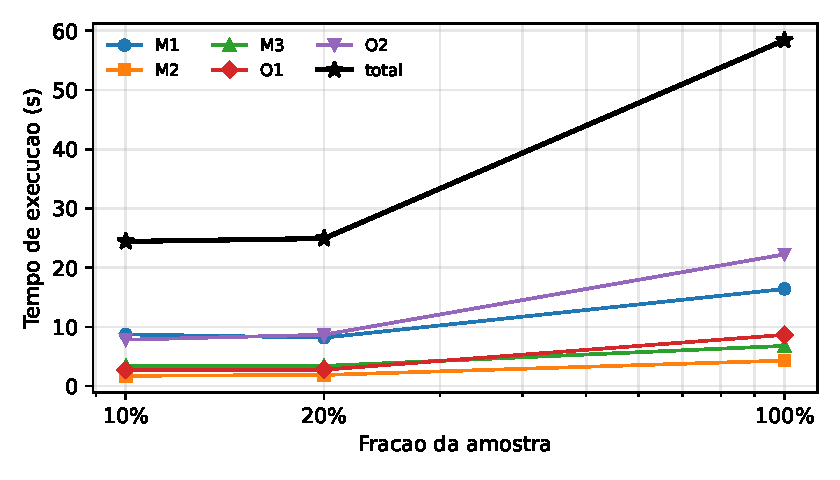
\includegraphics[width=\columnwidth]{fig_scale.pdf}
\caption{Tempo de execução por operação em função da fração da amostra
(variante final, \texttt{local[*]}).}
\label{fig:scale}
\end{figure}

\subsection{Escala do dataset}

Corri o pipeline otimizado em amostras de 10\%, 20\% e 100\%. A
Figura~\ref{fig:scale} mostra que o crescimento é sub-linear: 10 vezes
mais dados produzem apenas 2.4 vezes mais tempo (24.4 s, 24.9 s e 58.4 s
de soma das operações). Duas causas se destacam. Em frações pequenas, os
custos fixos dominam: arranque da JVM, planeamento de consultas e
agendamento de \emph{tasks} são constantes, pelo que entre 10\% e 20\%
os tempos quase não se alteram. No M1 a 100\%, a materialização do
\emph{cache} passa a pressionar a memória (3.5 GB de dados limpos), o que
explica o salto de 8.2 s para 16.4 s; as restantes operações mantêm
proporcionalidade aproximada.

\subsection{Tamanho do cluster}

Sem acesso ao cluster DI, aproximei o escalonamento por nós correndo o
pipeline com 4 \emph{cores} (\texttt{local[4]}) e com as 16 \emph{threads}
disponíveis. A Figura~\ref{fig:speedup} reporta o speedup
$T_4/T_{16}$. No O2, a operação dominante, o speedup é 1.46$\times$ para
um ideal de 4$\times$ (eficiência de 36\%). Os desvios face ao speedup
ideal têm causas identificáveis: as 16 \emph{threads} correspondem a 8
núcleos físicos com \emph{hyperthreading}; a largura de banda de memória
e de disco é partilhada entre os \emph{cores}, e a agregação do O2 é
intensiva em ambas; e o AQE coalesce partições de shuffle, reduzindo o
paralelismo efetivo. No M2 o speedup é de 1.34$\times$ e quase todo o
seu tempo é leitura do \emph{cache} em memória e agregação de 0.7 MB de
shuffle, ou seja, está limitado por I/O e não por computação.

\begin{figure}[t]
\centering
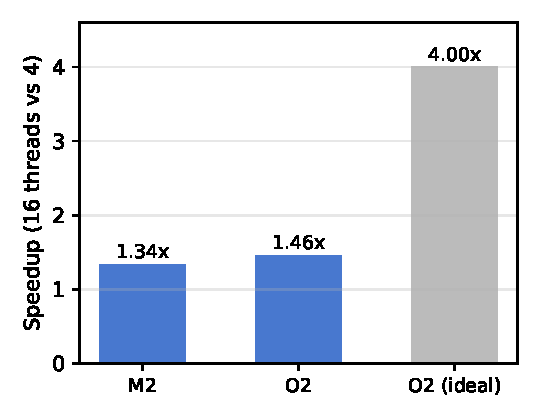
\includegraphics[width=0.7\columnwidth]{fig_speedup.pdf}
\caption{Speedup das operações dominantes entre 4 e 16 \emph{threads}.}
\label{fig:speedup}
\end{figure}

\section{Discussão}

Restam gargalos por endereçar. O O2 é o mais pesado e o seu custo está
na agregação por (origem, destino, mês) sobre 35 milhões de linhas;
técnicas de \emph{salting} para a assimetria das zonas de aeroporto ou o
ajuste fino do AQE para \emph{skewed joins} seriam os passos seguintes,
mas a assimetria medida (razão máximo/mediana de 4.4$\times$) ainda não
justifica a complexidade. A tentativa de \emph{persist} do intermédio
do O2 (74 s, 5815 \emph{tasks}) mostrou que mais \emph{cache} não é
sempre melhor: o intermédio é grande o suficiente para competir com o
\emph{cache} do M1 pela memória do \emph{driver}, e o recomputar barato
de um plano linear vence. É também uma limitação da metodologia: em modo
local, executor e \emph{driver} partilham memória, e o \emph{cache} em
modo local comporta-se de forma diferente de um cluster.

Há limitações a registar. A métrica de \emph{input bytes} da Spark UI
mostrou-se pouco fiável em modo local (por exemplo, \texttt{count()} em
Parquet usa os metadados do rodapé e lê quase nada), pelo que baseei as
conclusões em tempos de parede, tempo de CPU e bytes de shuffle, e
capturei os planos físicos em texto em vez de capturas de ecrã. As
corridas têm ruído de 10 a 20\% entre processos, daí as comparações
A/B terem sido feitas sempre em processos novos e emparelhados. Com mais
tempo, correria o estudo completo no cluster Docker do laboratório com
dois tamanhos de alocação, estenderia o dataset a mais anos (o código já
aceita vários anos como argumento) e exploraria o O3, cujo auto-join com
desfasamento temporal é o candidato natural a um sexto estudo de
otimização.

\bibliographystyle{acm}
\bibliography{refs}

\appendix
\section*{Página extra}

A bibliografia segue no fim do documento (ficheiro \texttt{refs.bib}).

\subsection*{Agradecimentos}

\paragraph{Onde usei IA.}
Usei o assistente Kimi em três situações. A primeira foi a geração de
uma primeira versão do código do pipeline (leitura dos CSVs, agregações
de M1 a M3, escrita de CSVs), que depois ajustei, corrigi e validei
correndo localmente contra os dados reais. A segunda foi a depuração de
problemas de ambiente: o PySpark no Windows precisa do \texttt{hadoop.dll}
e do \texttt{winutils.exe}, e as primeiras corridas falhavam com erros
pouco claros; o assistente ajudou-me a perceber que o \texttt{java.library.path}
é montado a partir do \texttt{PATH} e que era isso que estava a falhar,
o que originou o script \texttt{run.sh}. A terceira foi na revisão de
partes do texto deste relatório (clareza, português e formatação
LaTeX).

\paragraph{Exemplos de instruções que dei.}
Escrevi sempre em linguagem natural, por exemplo: ``escreve um script
PySpark que lê os CSVs do NYC Taxi e calcula três agregações'';
``o Spark dá JAVA\_GATEWAY\_EXITED no meu Windows, como resolvo?'';
``reescreve esta secção do relatório de forma mais simples''. Não
coloquei instruções complexas nem modelos; foi sempre conversa direta.

\paragraph{Agente.}
Não desenvolvi nenhum agente. Toda a interação foi por instruções
em texto, uma a uma.

\paragraph{Ligação às métricas.}
Cada otimização do trabalho foi decidida por mim a partir dos números
do \texttt{resumo.json} e dos planos físicos do Spark UI, como se descreve
na secção de estudo de otimização (variantes \texttt{final},
\texttt{nobroadcast}, etc.). A IA serviu para produzir código de partida
e para explicar erros, não para tomar decisões de otimização nem para
interpretar resultados. Todas as corridas e medições foram feitas por mim
nesta máquina, e os valores do relatório provêm dos ficheiros em
\texttt{results/}, reproduzíveis com os comandos do README.

\subsection*{Contribuições individuais}
Trabalho realizado individualmente por Rodrigo Mira (n.\textsuperscript{o}
79432): conceção do pipeline, implementação, experiências, análise e
redação, 100\%.

\subsection*{Comentários e sugestões}
O ciclo perfilar-otimizar-medir funcionou bem, mas o cluster DI
indisponível limitou a componente de escalabilidade; seria útil que o
acesso ao cluster estivesse garantido durante o projeto. O profiler do
Lab 3 em formato de API REST foi a ferramenta mais valiosa do trabalho.

\end{document}
